\documentclass[11pt]{article}
\usepackage[margin=1in]{geometry}
\usepackage{amsmath, amsfonts}
\usepackage[noend]{algpseudocode}
\usepackage{algorithm}
\usepackage[parfill]{parskip}
\usepackage{enumerate}
\usepackage[shortlabels]{enumitem}
\usepackage{hyperref}
\usepackage[english]{babel}
\usepackage[autostyle]{csquotes}
\usepackage{enumitem}
\usepackage{wrapfig}
\usepackage{tikz}
\usetikzlibrary{decorations.pathreplacing}
\definecolor{color1}{rgb}{0.7, 0.2, 0.2}
\definecolor{color2}{rgb}{0.0, 0.4, 0.0}
\definecolor{color3}{rgb}{0.2, 0.4, 0.7}

%--------------------------------------------------------%


\title{\vspace{-0.5in}Compsci 330 Design and Analysis of Algorithms \\Assignment 5, Spring 2024 Duke University}
\author{TODO: Add your name(s) here}
\date{Due Date: Thursday, February 22, 2024}

%--------------------------------------------------------%

\begin{document}

\maketitle


%--------------------------------------------------------%

\paragraph{How to Do Homework.} We recommend the following three step process for homework to help you learn and prepare for exams.
\begin{enumerate}
	\item Give yourself ~15-20 minutes per problem to try to solve on your own, without help or external materials, as if you were taking an exam. Try to brainstorm and sketch the algorithm for applied problems. Don't try to type anything yet.
	\item After a break, review your answers. Lookup resources or get help (from peers, office hours, Ed discussion, etc.) about problems you weren't sure about.
	\item Rework the problems, fill in the details, and typeset your final solutions.
\end{enumerate}

\paragraph{Typesetting and Submission.} Your solutions should be typed and submitted as a single pdf on Gradescope. Handwritten solutions or pdf files that cannot be opened will not be graded. \LaTeX \footnote{If you are new to \LaTeX, you can download it for free at \href{https://www.latex-project.org}{latex-project.org} or you can use the popular and free (for a personal account) cloud-editor \href{https://www.overleaf.com}{overleaf.com}. We also recommend \href{https://www.overleaf.com/learn}{overleaf.com/learn} for tutorials and reference.} is preferred but not required. %If you use another editor for your solutions (such as Microsoft Word), you should convert the final document to a pdf, confirm that the symbolic math from the equation editor is properly formatted, and submit the pdf. 
You must mark the locations of your solutions to individual problems on Gradescope as explained in \href{https://help.gradescope.com/article/ccbpppziu9-student-submit-work#submitting_a_pdf}{the documentation}. Any applied problems will request that you submit code separately on Gradescope to be autograded. 

\paragraph{Writing Expectations.} If you are asked to provide an algorithm, you should clearly and unambiguously define every step of the procedure as a combination of precise sentences in plain English or pseudocode. If you are asked to explain your algorithm, its runtime complexity, or argue for its correctness, your written answers should be clear, concise, and should show your work. Do not skip details but do not write paragraphs where a sentence suffices.

\paragraph{Collaboration and Internet.} If you wish, you can work with a single partner (that is, in groups of 2), in which case you should submit a single solution \href{https://help.gradescope.com/article/m5qz2xsnjy-student-add-group-members}{as a group on gradescope}. You can use the internet, but looking up solutions or using large language models is unlikely to help you prepare for exams. See the \href{https://sites.duke.edu/spring24compsci330/policies/}{course policies webpage} for more details.

\paragraph{Grading.} Theory problems will be graded by TAs on an S/U scale (for each sub-problem). Applied problems typically have a separate autograder where you can see your score. The lowest scoring problem is dropped. See the \href{https://sites.duke.edu/spring24compsci330/assignments/}{course assignments webpage} for more details.



%--------------------------------------------------------%


\newpage
\paragraph{Problem 1 (DAG Reachability).} You are given a directed acyclic graph $G = (V, E)$ with $n$ vertices and $m$ edges, in which each node $u \in V$ has an associated {\em price} $p_u$ which is a positive integer. Define the array {\sc cost} as follows: For each $u \in V$,
$$\textsc{cost}[u] = \text{price of the cheapest node reachable from }u 
 \text{ (including }u\text{ itself)}.$$
 For instance, in the graph below (with prices shown for each vertex), the {\sc cost} values of the nodes $A$, $B$, $C$, $D$, $E$, $F$ are $2, 1, 4, 1, 4, 5$, respectively.

\begin{figure}[!h]
\centering
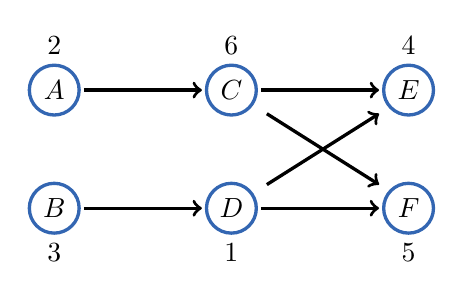
\begin{tikzpicture}[yscale = 0.75, xscale = 0.75]

\draw [very thick, color3] (-3, 1) circle (12pt);
\draw [very thick, color3] (-3, -1) circle (12pt);
\draw [very thick, ->] (-2.5, 1) -- (-0.5, 1);
\draw [very thick, ->] (-2.5, -1) -- (-0.5, -1);
\draw [very thick, color3] (0, 1) circle (12pt);
\draw [very thick, color3] (0, -1) circle (12pt);
\draw [very thick, ->] (0.5, 1) -- (2.5, 1);
\draw [very thick, ->] (0.5, -1) -- (2.5, -1);
\draw [very thick, ->] (0.6, 0.6) -- (2.5, -0.6);
\draw [very thick, ->] (0.6, -0.6) -- (2.5, 0.6);
\draw [very thick, color3] (3, 1) circle (12pt);
\draw [very thick, color3] (3, -1) circle (12pt);
\node at (-3, 1.75) {$2$}; \node at (0, 1.75) {$6$};
\node at (3, 1.75) {$4$}; \node at (-3, -1.75) {$3$};
\node at (0, -1.75) {$1$}; \node at (3, -1.75) {$5$};
\node at (-3, 1) {$A$}; \node at (-3, -1) {$B$};
\node at (0, 1) {$C$}; \node at (0, -1) {$D$};
\node at (3, 1) {$E$}; \node at (3, -1) {$F$};

\end{tikzpicture}
\end{figure}
 
Describe an algorithm that completes the {\em entire} {\sc cost} array (i.e., for all vertices) in $O(m + n)$ time. Briefly explain the correctness of the algorithm and analyze its runtime complexity.

You may use depth-first search (DFS) or Kosaraju's SCC algorithm as described in lecture without restating the algorithm or arguing for its correctness.

\paragraph{Solution}
For this solution, we will assume that line 3 (that is, the call to \Call{dfs}{})
updates the \texttt{price} array such that \texttt{price[n] = n.price}, where
$n$ is the identity of the node. Also, we will let $ \text{topo}^{R}$ denote
traversal in reverse-topological order.

\begin{algorithm}
\caption{Problem 1 solution}
\begin{algorithmic}[1]
\Procedure{findCost}{$G$}
\State cost = [$\infty$]
\Comment{initialize cost with value $\infty$ at all elements}
\State price = []
\State topo = \Call{dfs}{$G$}
\Comment{updates \texttt{price} array}
\For{$u$ in topo$^{R}$}
\Comment{reverse-topological traversal}
    \State min\_cost = price[$u$]
    \For{every edge $u\rightarrow v$}
        \State min\_cost = \Call{min}{min\_cost, cost[$v$]}
    \EndFor
    \State cost[$u$] = min\_cost
\EndFor
\State \Return cost
\EndProcedure 
\end{algorithmic}
\end{algorithm}

Going in reverse toplological order starts with a sink node, whose cost is its
own price by definition (since it has out-degree 0). After the sink, because the
cost of a node is the lowest price reachable from that node, we only need to
check immediately adjacent nodes' costs and compare to the current node to find
the minimum reachable price (i.e. the cost). After doing this for all nodes,
we arrive at our solution.

Our depth-first search takes $O(n+m)$ time. Because we only traverse a constant
number of nodes at each iteration of our reverse-topological traversal, this
also takes $O(n+m)$ time. Thus, our final runtime is
\[
    O(n+m) + O(n+m) = O(n+m+n+m) = O(2n + 2m) = \boxed{O(n+m)}.
\]


%--------------------------------------------------------%
\newpage
\paragraph{Problem 2 (Dining Preferences).} Suppose $m$ friends want to eat dinner together and there are $n$ possible restaurants to choose from. Each friend $k$ reports an array $A_k$ of length $n_k \leq n$ where each element is a restaurant, and $A_k$ is sorted in decreasing order of preferred restaurants for the friend $k$. Set $N = \sum_{i=1}^k n_i$. Describe an $O(n+N)$-time algorithm that either computes an array $B$ of length $n$ sorted in a way that is consistent with the preference of all of the friends or reports that none exists. That is, 
for all $1\le k \le m$ and $1 \le j < n_k$, $A_k[j]$ appears before $A_k[j+1]$ in $B$, or reports that no such ordering exists. 

For example, suppose there are three restaurants and three friends, and their preferences are $A_1 = [a,c], A_2 = [c,b] \text{ and } A_3 = [a,b]$. Then $(a,c,b)$ is a valid ordering of the three restaurants.

Briefly explain the correctness of the algorithm and analyze its runtime complexity.

You may use depth-first search (DFS) or Kosaraju's SCC algorithm as described in lecture without restating the algorithm or arguing for its correctness.

\paragraph{Solution}
We will let $A$ be a 2-dimensional array , where each element $k$ contains
$A_{k}$. Additionally, assume that the \texttt{visited} array has been declared
globally for ease of use. We will state that our \Call{findPrefs}{} procedure
will return 0 to denote that no solution exists.

\begin{algorithm}
\caption{Problem 2 solution}
\begin{algorithmic}[1]
\Procedure{generateEdgeList}{$A$}
    \State $E = []$
    \Comment{edge list}
    \For{$k$ in $1\rightarrow m$}
        \State prefs = []
        \State $A_{k} = A[k]$
        \For{$p$ in $1 \rightarrow n-1$}
            \State prefs[$p-1$] = ($A_{k}[p-1], A_{k}[p]$)
        \EndFor
        \State $E[k-1] =$ prefs
    \EndFor
\EndProcedure

\Procedure{hasBackEdge}{$G$}
    \State visited = []
    \For{$u \in G$}
        \State visited[$u$] = True
        \For{each edge $u\rightarrow v$}
            \If{visited[$v$]}
                \State \Return True
            \EndIf
        \EndFor
    \EndFor
    \State \Return False
\EndProcedure 

\Procedure{findPrefs}{$A$}
    \State $G$ = \Call{generateEdgeList}{$A$}
    \State topo = \Call{dfs}{$G$}
    \Comment{create topological ordering from edge list using DFS}
    \If{\Call{hasBackEdge}{topo}}
        \State \Return 0
    \Else
        \State \Return topo
    \EndIf
\EndProcedure 
\end{algorithmic}
\end{algorithm}

Here we first construct the graph from an edge list provided. We then put that
graph into topological order using \Call{dfs}{}, for which we are told to assume
correctness. If that topological ordering contains a back edge, then no
solution exists, since at least two friends have mutually conflicting 
preferences. Fortunately, if no back edges exist, then the toplogical ordering
is the correct ordering of preferences, with the source node being the most
preferred location among the correct ordering, and the sink node being the
least preferable.

To create the graph, we have to do iterate through all $k$ friends list of
$n$ restaurants. That requires $O(kn)$ time. Topological ordering with DFS 
takes $O(N+n)$ time. Thus, we have
\[
    O(kn) + O(N+n) = O(kn + N + n) = O((k+1)n + N) = \boxed{O(kn + N)}.
\]


%--------------------------------------------------------%

\newpage
\paragraph{Problem 3 (Transit Connections).} The NotUnited airline company operates in locations numbered $1, 2, \dots, n$ and is based in location $1$. NotUnited offers $m$ connections between these locations. These connections are specified by a list of tuples where $(i, j)$ means that there is a connection from location $i$ to $j$. Connections are one way.

NotUnited guarantees that it is possible to reach all $n-1$ additional operating locations via connections (possibly more than one) originating at their base in location $1$. However, some customers have complained about finding themselves unable to return home via NotUnited connections after traveling to another destination. Describe an $O(n+m)$ runtime algorithm to compute the minimum number of connections that the company would need to add in order to ensure that this cannot happen. Briefly explain the correctness of the algorithm and analyze its runtime complexity.

You may use depth-first search (DFS) or Kosaraju's SCC algorithm as described in lecture without restating the algorithm or arguing for its correctness.

\paragraph{Solution 3 (Description)}

This problem is actually relatively straightforward, so we will write it in a somewhat informal explanation:

\begin{enumerate}
    \item Run Kosaraju's SCC algorithm to identify all of the SCCs. Specifically, identify components which are sinks and components which are sources. This can be accomplished by running SCC on both the original graph and the reverse graph. For this algorithm, a quantity is sufficient.
    \item The minimum number of connections needed to add in order to ensure everyone is able to run home is simply the maximum number of sink or source components in the condensation (e.g., if there are two sink components and three source components, the minimum number of connections needed is 3).
\end{enumerate}

\paragraph{Solution 3 (Explanation of Correctness)}

Running Kosaraju's SCC algorithm allows us to understand the condensation of a graph. Within any SCC, it is possible for passengers to get between any two locations, so no connections need to be added within an SCC. Thus, all we need to do is connect the different SCCs (i.e., the ``nodes" of the condensation).
\vspace{0.5em}

A very simple solution to this problem is to connect sink nodes to source nodes. The graph is connected, so every source component can reach at least one other component, and every sink component can be reached by at least one other component. If we can connect sink components back to source components, we can create a cycle, which enables everyone to be able to return home via connections (albeit sometimes in a very inefficient manner). We can fully connect the condensation by connecting each sink component to at least one source component (and ensuring that every sink component is connected to a source component). Thus, the number of connections needed is simply the maximum number of sink or source components (to ensure that there is at least one connection for each of these components). Any component that is neither a sink nor a source component can already be reached from some component and reach another component, so they do not need additional connections. 

\paragraph{Solution 3 (Runtime Complexity)}

We know, from explanations in the lecture notes, that Kosaraju's SCC algorithm can be run in $O(n + m)$ time if we do not need to explicitly sort vertices. In this case, since we only need the number of sink and source components, we are not concerned with any sorting. Thus, all that we need to do is run Kosaraju's SCC algorithm twice (once on the regular graph and once on the reverse graph, to find all source and sink components). After that, we are simply doing one mathematical comparison, which runs in constant time. Thus, this algorithm runs in $O(n + m)$ time.

%--------------------------------------------------------%

\newpage
\paragraph{Problem 4 (Applied).} You are given a computer network represented as a connected undirected graph $G=(V, E)$ where computers and routers are the vertices and connections between them are the edges. Say that a node in this network is a \textit{critical point} if removing the node (and its incident edges) increases the number of connected components in the network (for example, if it disconnects the network). For example, in the following diagram, $3$ and $5$ are both critical points.

\begin{figure}[!h]
\centering
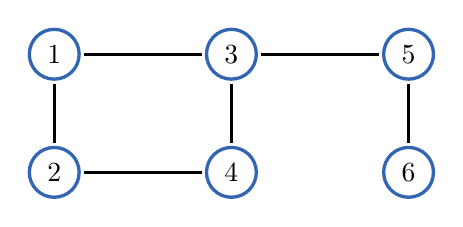
\begin{tikzpicture}[yscale = 0.75, xscale = 0.75]

\draw [very thick, color3] (-3, 1) circle (12pt);
\draw [very thick, color3] (-3, -1) circle (12pt);
\draw [very thick, -] (-2.5, 1) -- (-0.5, 1);
\draw [very thick, -] (-2.5, -1) -- (-0.5, -1);
\draw [very thick, color3] (0, 1) circle (12pt);
\draw [very thick, color3] (0, -1) circle (12pt);
\draw [very thick, -] (0.5, 1) -- (2.5, 1);
\draw [very thick, -] (0, 0.5) -- (0, -0.5);
\draw [very thick, -] (-3, 0.5) -- (-3, -0.5);
\draw [very thick, -] (3, 0.5) -- (3, -0.5);
\draw [very thick, color3] (3, 1) circle (12pt);
\draw [very thick, color3] (3, -1) circle (12pt);
\node at (-3, 1) {$1$}; \node at (-3, -1) {$2$};
\node at (0, 1) {$3$}; \node at (0, -1) {$4$};
\node at (3, 1) {$5$}; \node at (3, -1) {$6$};

\end{tikzpicture}
\end{figure}

You will need to \textbf{design and implement} an algorithm that returns a list of all the critical points (as ints) in \textbf{any order} in $O(n+m)$ time (where $n=|V|$ and $m=|E|$). 

Language-specific details follow. You can use whichever of Python or Java you prefer. You will receive automatic feedback when submitting, and you can resubmit as many times as you like up to the deadline. \textbf{NOTE:} Unlike the theory problems, the applied problem grade \textbf{is the raw score shown on Gradescope}. See the \href{https://sites.duke.edu/spring24compsci330/assignments/}{course assignments webpage} for more details. 

\begin{itemize}
	\item \textbf{Python.} You should submit a file called \texttt{critical.py} to the Gradescope item ``Homework 5 - Applied (Python).'' The file should define (at least) a top level function \texttt{critical} that takes in two inputs, an int $n$, which defines the number of vertices, and a list of tuples \texttt{(i:int, j:int)} \texttt{edges} where \texttt{(i,j)} refers to an undirected edge from node \texttt{i} to node \texttt{j} and return a list of \texttt{int} where each element is one of the critical points of the graph (in any order). The function header is as follows
    \begin{itemize}
        \item \texttt{def critical(n:int, edges:list[(int, int)]):}
    \end{itemize}
	
    \item \textbf{Java.} You should submit a file called \texttt{Critical.java} to the Gradescope item ``Homework 5 - Applied (Java)'' The file should define (at least) a top level function \texttt{critical} that takes in one 2D int array: \texttt{edges} and returns an ArrayList$<$Integer$>$ where each element is one of the critical points of the graph (in any order). The header for the method is as follows
    \begin{itemize}
        \item \texttt{public ArrayList<Integer> critical(int n, int[][] edges);}
    \end{itemize}
    edges is a $k$ by 2 2D arrays, where edges$[i]$ is the undirected edge from edges$[i][0]$ to edges$[i][1]$

\end{itemize}

\textbf{Hint.} To begin, consider the depth-first search tree of the graph. For the root of the search tree, how can you tell if it is a critical point? For the other nodes, how can you tell by looking at the back edges of the tree? Finally, how can you use the pre-visit times to solve the problem in linear time?

\end{document}
